%%%%%%%%%%%%%%%%%%%%%%%%%%%%%%%%%%%%%%%%%%%%%%%%%%%%%%%%%%%%%%%%%%%%%%%%%%%%%%%%
% AMS Beamer series / Bologna FC / Template
% Andrea Omicini
% Alma Mater Studiorum - Università di Bologna
% mailto:andrea.omicini@unibo.it
%%%%%%%%%%%%%%%%%%%%%%%%%%%%%%%%%%%%%%%%%%%%%%%%%%%%%%%%%%%%%%%%%%%%%%%%%%%%%%%%
%\documentclass[handout]{beamer}\mode<handout>{\usetheme{default}}
%
\documentclass[presentation, 9pt]{beamer}\mode<presentation>{\usetheme{AMSBolognaFC}}
%\documentclass[handout]{beamer}\mode<handout>{\usetheme{AMSBolognaFC}}
%%%%%%%%%%%%%%%%%%%%%%%%%%%%%%%%%%%%%%%%%%%%%%%%%%%%%%%%%%%%%%%%%%%%%%%%%%%%%%%%
\usepackage[T1]{fontenc}
\usepackage{wasysym}
\usepackage{amsmath,blkarray}
\usepackage[minted,most]{tcolorbox}
\usepackage{centernot}
\usepackage{fontawesome}
\usepackage{tasks}
\usepackage{fancyvrb}
\usepackage{minted}
\usepackage{hyperref}
\usepackage{multicol}
\setminted[scala]{fontsize=\scriptsize,baselinestretch=1,obeytabs=true, tabsize=2}
\usepackage[ddmmyyyy]{datetime}
\setminted{fontsize=\footnotesize}
\renewcommand{\dateseparator}{}
%\renewcommand{\thefootnote}{\fnsymbol{footnote}}
\newcommand{\version}{1}
\usepackage[
	backend=biber,
	citestyle=authoryear-icomp,
	maxcitenames=1,
	bibstyle=numeric]{biblatex}

	\makeatletter

\addbibresource{biblio.bib}
%%%%%%%%%%%%%%%%%%%%%%%%%%%%%%%%%%%%%%%%%%%%%%%%%%%%%%%%%%%%%%%%%%%%%%%%%%%%%%%%
\title[Advanced Topics in Reinforcement Learning]
{Advanced Topics in Reinforcement Learning}
%
\subtitle[Deep Learning and Multi Agent Systems]
{Deep Learning and Multi Agent Systems}
%
\author[\sspeaker{Aguzzi}]
{\speaker{Gianluca Aguzzi} \href{mailto:gianluca.aguzzi@unibo.it}{gianluca.aguzzi@unibo.it}}
%
\institute[DISI, Univ.\ Bologna]
{Dipartimento di Informatica -- Scienza e Ingegneria (DISI)\\
\textsc{Alma Mater Studiorum} -- Universit{\`a} di Bologna \\[0.5cm]
\textbf{Talk @} \bold{Advanced Software Modelling and Design}}
%
\renewcommand{\dateseparator}{/}
\date[\today]{\today}
%
\AtBeginSection[]
{
  \begin{frame}
  \frametitle{Contents}
  \tableofcontents[currentsubsection, 
	sectionstyle=show/shaded, 
	subsectionstyle=show/shaded]
  \end{frame}
}
\AtBeginSubsection[]
{
  \begin{frame}
  \frametitle{Contents}
  \tableofcontents[currentsubsection, 
	sectionstyle=show/shaded, 
	subsectionstyle=show/shaded]
  \end{frame}
}
%%%%%%%%%%%%%%%%%%%%%%%%%%%%%%%%%%%%%%%%%%%%%%%%%%%%%%%%%%%%%%%%%%%%%%%%%%%%%%%%
\begin{document}
%%%%%%%%%%%%%%%%%%%%%%%%%%%%%%%%%%%%%%%%%%%%%%%%%%%%%%%%%%%%%%%%%%%%%%%%%%%%%%%%

\maketitle

%===============================================================================
\section{Introduction}
\begin{frame}{Introduction}
	\begin{itemize}
		\item \textbf{Reinforcement Learning (RL)} is a subfield of \emph{machine learning} that focuses on learning how to act in order to maximize a numerical reward signal
		\item Someone argues~\cite{SILVER2021103535} that reward maximization is the \textbf{sole} principle that suffices to explain all aspects of intelligent behavior
		\item Key features:
		\begin{itemize}
			\item \textbf{trial-and-error search} (no supervisor)
			\item \textbf{delayed reward} (no immediate feedback)
			\item \textbf{sequential decision-making} (the current decision affects the future decisions)
		\end{itemize}
		\item \textbf{Today lesson}
		\begin{itemize}
			\item Scale to more complex problems \faArrowRight \, \textbf{Deep Reinforcement Learning}
			\item Scale to multi-agent systems \faArrowRight \, \textbf{Multi-Agent Reinforcement Learning}
		\end{itemize}
	\end{itemize}
\end{frame}
\section{Deep Reinforcement Learning}
%===============================================================================
%\subsection{Reinforcement Learning Pitfalls}
\begin{frame}{\textbf{Road to deep}: Large state space}
\begin{block}{Problem}
	\begin{itemize}
		\item \textbf{State-space} \faArrowRight \, set of all possible states
		\item \textbf{State-space explosion} \faArrowRight \, the number of states is too large to be stored in memory
	\end{itemize}
\end{block}
\begin{columns}
	\begin{column}{0.5\textwidth}
		
			\begin{block}{Example (Go) \, \href{}{\faLink}}
				\begin{itemize}
					\item $10^{170}$ possible states \bold{(!!!!)}
					\item $10^{80}$ atoms in the universe
					\item $10^{16}$ seconds since the Big Bang
				\end{itemize}
			\end{block}
			\begin{block}{Example (Chess) \, \href{}{\faLink}}
				\begin{itemize}
					\item $10^{46}$ possible states
					\item total space required $\sim$ $10^{35}$ terabytes
				\end{itemize}
			\end{block}
	\end{column}
	\begin{column}{0.5\textwidth}
	\centering
	\fbox{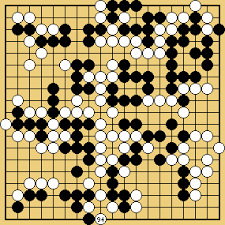
\includegraphics[width=0.67\linewidth]{img/go.png}}
	\end{column}
\end{columns}

\begin{alertblock}{Question}
	\centering
	\textbf{How can we effectively handle large state spaces?}
\end{alertblock}
\end{frame}

\begin{frame}{Road to \textbf{Deep}: Continous Action Space}
	\begin{block}{Problem}
		\begin{itemize}
			\item \textbf{Action space} \faArrowRight \, set of all possible actions
			\item \textbf{Continous action space} \faArrowRight \, the actions are real numbers (e.g. $[0,1]$) \faArrowRight infinite number of actions
		\end{itemize}
	\end{block}
	\begin{columns}
		\begin{column}{0.5\textwidth}
			\begin{block}{Example (Robotics) \, \href{}{\faLink}}
				\begin{itemize}
					\item \textbf{Action space} \faArrowRight \, the set of all possible joint angles
					\item \textbf{Continous action space} \faArrowRight \, the set of all possible real joint angles
				\end{itemize}
			\end{block}
		\end{column}
		\begin{column}{0.5\textwidth}
			\centering
			\fbox{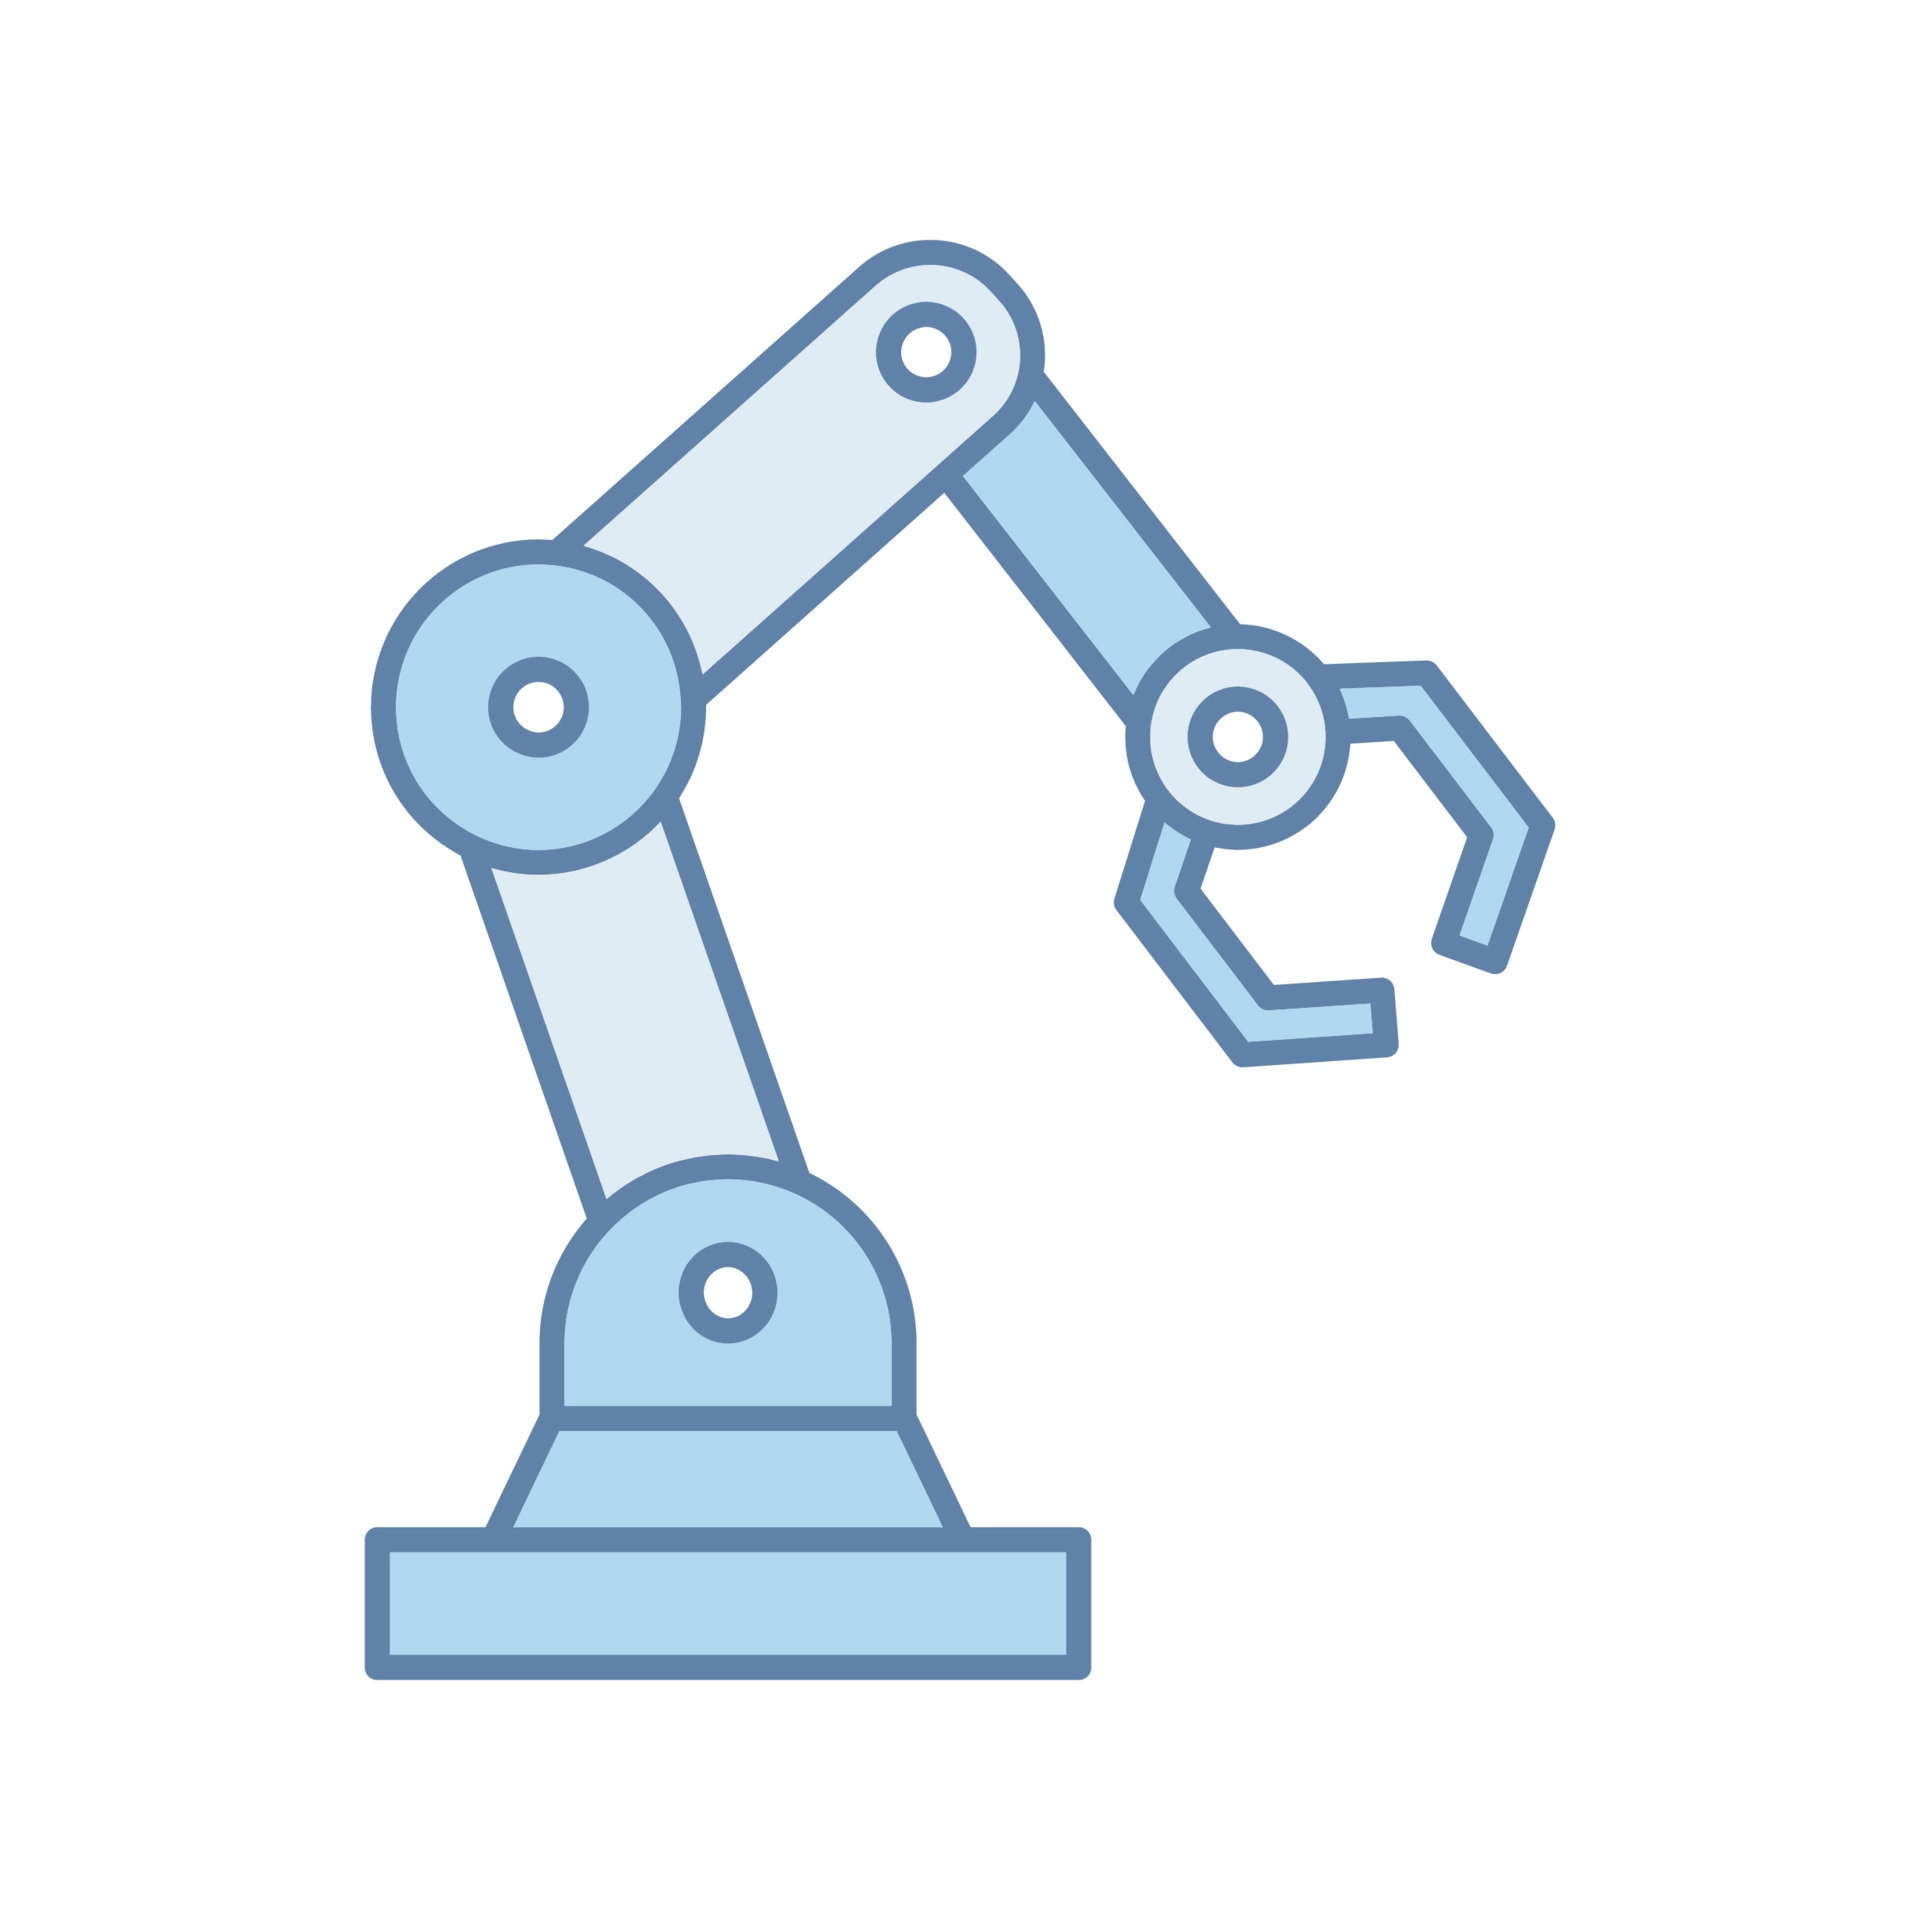
\includegraphics[width=0.4\linewidth]{img/robotics}}
		\end{column}
	\end{columns}
	
	\begin{alertblock}{Question}
		\centering
		\textbf{How can we effectively handle continuous action space?}
	\end{alertblock}
\end{frame}
\begin{frame}{Road to \textbf{Deep}: Generalization}
\begin{block}{Problem}
	\begin{itemize}
		\item \textbf{Generalization} \faArrowRight \, the ability to perform well on unseen environments beyond the training set
		\item Can be also seen as \textbf{transfer learning} \faArrowRight \, the ability to transfer knowledge from one environment to another
		\item \textbf{Generalization gap} \faArrowRight \, the difference between the performance on the training environments and the performance on the test environments
	\end{itemize}
\end{block}
\begin{block}{Example (Go)}
	\begin{itemize}
		\item \textbf{Generalization} \faArrowRight \, the ability to play well with different opponents
		\item \textbf{Generalization gap} \faArrowRight \, the difference between the performance on the training set and the performance on the test set
	\end{itemize}
\end{block}
\begin{alertblock}{Question}
	\centering
	\textbf{How to deal with generalization?}
\end{alertblock}
\end{frame}
%\subsection{Deep Reinforcement Learning Overview}
\begin{frame}{Deep Reinforcement Learning}
	\centering
	\fbox{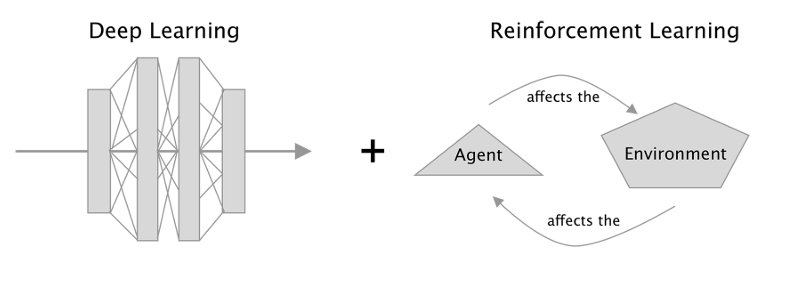
\includegraphics[width=0.7\textwidth]{img/deep-rl.png}}
	\begin{block}{Overview}
		\begin{itemize}
			\item \textbf{Deep Reinforcement Learning (DRL)} \faArrowRight \, the use of deep neural networks to approximate the value function / policy
			%\item Stochastic gradient descent \faArrowRight \, the use of gradient descent to train the neural networks
		\end{itemize}
	\end{block}
	
	\begin{alertblock}{Key features}
		\begin{itemize}
			\item \textbf{Value function approximation} (instead of tables) \faArrowRight \, \textbf{handle large state space}
			\item \textbf{Policy gradient} (instead of Q-Learning) \faArrowRight \, \textbf{handle continous action space}
			\item \textbf{Deep neural networks} \faArrowRight \, \textbf{handle generalization} (Representation learning)
		\end{itemize}
	\end{alertblock}
\end{frame}
\begin{frame}{Algorithms types}	
\begin{columns}
	\begin{column}{0.45\textwidth}
		\begin{block}{Value-based}
			\begin{itemize}
				\item the agent learns the value function
				\item \textbf{Example} \faArrowRight \, \emph{Deep Q-Learning}
			\end{itemize}
		\end{block}
		\href{https://www.youtube.com/watch?v=V1eYniJ0Rnk}{\fbox{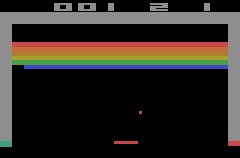
\includegraphics[height=3.5cm]{img/atari}}}
	\end{column}

	\begin{column}{0.45\textwidth}
		\begin{block}{Policy-based}
			\begin{itemize}
				\item The agent learns \emph{directly} the policy 
				\item \textbf{Example} \faArrowRight \, REINFORCE, PPO
			\end{itemize}
		\end{block}
		\centering
		\href{https://openai.com/research/openai-baselines-ppo}{\fbox{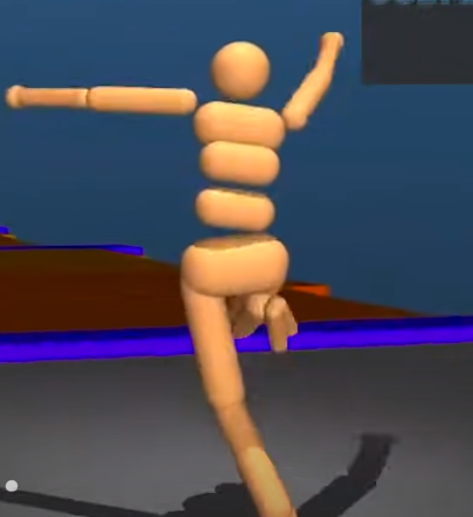
\includegraphics[height=3.5cm]{img/ppo.png}}}
	\end{column}
\end{columns}

\end{frame}
\begin{frame}{Deep Q-Learning -- in a nutshell}
	\centering
	\large{
	\textbf{Q-Learning but the q-table is approximated by a neural network}
	}
	$$ Q(s, a, \theta) \sim Q(s, a) $$
	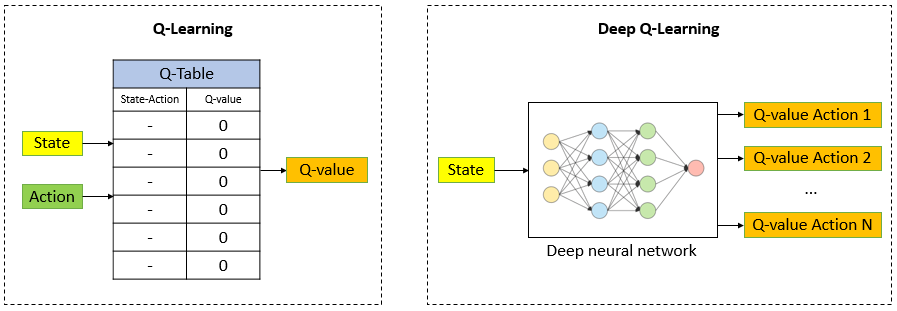
\includegraphics[width=\textwidth]{img/dql-vs-ql-1.png}
\end{frame}

\begin{frame}{Deep Q-Learning}
	\begin{alertblock}{Loss function}
		\begin{itemize}
			\item Bellman equation: $Q(s, a) = (r + \gamma \max_{a'} Q(s', a'))$
			\item Treating $r + \gamma \max_{a'} Q(s', a')$ as a target value
			\item Regression problem: $L(\theta) = (r + \gamma \max_{a'} Q(s', a', \theta) - Q(s, a, \theta))^2$
		\end{itemize}
	\end{alertblock}
	\begin{block}{Issues}
		\begin{itemize}
			\item \textbf{Correlation} \faArrowRight \, the samples are not independent
			\item \textbf{Non-stationary} \faArrowRight \, the target value changes over time
		\end{itemize}
	\end{block}
	\begin{alertblock}{Solutions}
		\begin{itemize}
			\item \textbf{Replay Buffer} \faArrowRight \, store the transitions $(s, a, r, s')$ and sample them randomly
			\item \textbf{Target Network} \faArrowRight \, used to compute the target value
		\end{itemize}
	\end{alertblock}
\end{frame}
\begin{frame}{Deep Q Learning: Replay Buffer}
	\centering
	\fbox{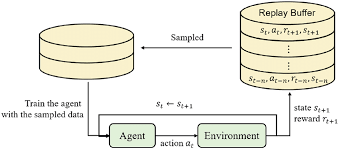
\includegraphics[width=0.5\textwidth]{img/replay-buffer.png}}
	\begin{block}{How}
		\begin{itemize}
			\item Store the transitions $(s, a, r, s')$ in $\mathcal{D}$ of prior experience
			\item During Backpropagation, sample a batch of transitions $(s, a, r, s')$ 
		\end{itemize}
	\end{block}
	\begin{block}{Loss computation}
		\begin{itemize}
			\item Sample a random batch of transitions $(s, a, r, s')$ from $\mathcal{D}$
			\item Compute the target value $y = r + \gamma \max_{a'} Q(s', a', \theta)$
			\item Use the target value to compute the loss $L(\theta) = \mathbb{E}[(y - Q(s, a, \theta))^2]$
		\end{itemize}
	\end{block}
\end{frame}
\begin{frame}{Deep Q Learning: Fixed Target Network}
	\centering
	%\fbox{\includegraphics[width=0.5\textwidth]{img/target-network.png}}
	\begin{block}{How}
		\begin{itemize}
			\item Use a separate network to compute the target value
			\item The target network is updated every $C$ steps
		\end{itemize}
	\end{block}
	\begin{block}{Loss computation}
		\begin{itemize}
			\item Let $\theta^-$ be the parameters of the target network
			\item Sample a random batch of transitions $(s, a, r, s')$ from $\mathcal{D}$
			\item Compute the target value $y = r + \gamma \max_{a'} Q(s', a', \theta^-)$
			\item Use the target value to compute the loss $L(\theta) = \mathbb{E}[(y - Q(s, a, \theta))^2]$
			\item After $C$ steps, update the target network parameters $\theta^- \leftarrow \theta$
		\end{itemize}
	\end{block}
	\begin{alertblock}{Benefits}
		\begin{itemize}
			\item \textbf{Stable} \faArrowRight \, the target value is fixed for $C$ steps, avoiding the non-stationary issue (dependence on target and prediction cause)
		\end{itemize}
	\end{alertblock}
\end{frame}
\begin{frame}{Deep Q Learning: Epsilon decay}
	\begin{block}{How}
		\begin{itemize}
			\item $\epsilon$ is the probability of selecting a random action
			\item $\epsilon$ is decayed over time (or steps or episodes)
			\item \textbf{(!!!)} Off-policy nature of DQL \faArrowRight \, the agent can learn from random actions
		\end{itemize}
	\end{block}
	\begin{block}{Why}
		\begin{itemize}
			\item \textbf{Exploration vs Exploitation} \faArrowRight \, the agent needs to explore the environment to learn the optimal policy
			\item \textbf{Exploitation} \faArrowRight \, the agent needs to exploit the learned policy to maximize the reward
		\end{itemize}
	\end{block}
	
\end{frame}
\begin{frame}{Deep Q Learning: Algorithm}
	\begin{block}{Algorithm}
		\begin{itemize}
			\item Initialize the replay buffer $\mathcal{D}$
			\item Initialize the target network parameters $\theta^-$
			\item Initialize the Q-network parameters $\theta$
			\item \textbf{for} episode = 1, M \textbf{do}
			\begin{itemize}
				\item Initialize the initial state $s_1$
				\item \textbf{for} t = 1, T \textbf{do}
				\begin{itemize}
					\item With probability $\epsilon$ select a random action $a_t$
					\item otherwise select $a_t = argmax_a Q(s_t, a, \theta)$
					\item Execute action $a_t$ in the environment and observe reward $r_t$ and next state $s_{t+1}$
					\item Store transition $(s_t, a_t, r_t, s_{t+1})$ in $\mathcal{D}$
					\item Sample a random minibatch of transitions $(s, a, r, s')$ from $\mathcal{D}$
					\item Set $y_i = r + \gamma \max_{a'} Q(s', a', \theta^-)$
					\item Perform a gradient descent step on $(y_i - Q(s, a, \theta))^2$ with respect to the network parameters $\theta$
					\item Every $C$ steps reset $\theta^- \leftarrow \theta$
				\end{itemize}
			\end{itemize}
		\end{itemize}
	\end{block}
\end{frame}
\begin{frame}{Deep Q Learning: Extensions and Limits}
	\begin{block}{Limits}
		\begin{itemize}
			\item Works only for discrete action spaces
			\item Sample inefficiencies
		\end{itemize}
	\end{block}
	\begin{block}{Extensions}
		\begin{itemize}
			\item \textbf{Double DQN} \faArrowRight \, use two separate networks to select and evaluate the action
			\begin{itemize}
				\item Pro: better estimation of the action value, reach higher performance
			\end{itemize}
			%\item \textbf{Dueling DQN} \faArrowRight \, use two separate networks to estimate the state value and the advantage function
			%\begin{itemize}
		%		\item Pro: better estimation of the action value
		%	\end{itemize}
			\item \textbf{Prioritized Experience Replay} \faArrowRight \, sample the transitions from the replay buffer according to their TD-error
			\begin{itemize}
				\item Pro: better exploration of the state space
			\end{itemize}
			\item \textbf{Raindow DQN} \faArrowRight \, combination of the previous extensions
		\end{itemize}
	\end{block}
\end{frame}
\begin{frame}[plain]
\begin{center}
	\Huge{\textbf{Code!}}
\end{center}
\centering
\small{\url{https://github.com/cric96/advanced-reinforcement-learning-asmd-code}}
\end{frame}
\section{Multi-Agent Reinforcement Learning}

\begin{frame}[c]{Multi-Agent Reinforcement Learning (MARL)}
	%/////////
	
	\begin{exampleblock}{Definition}
		\emph{Multiple} agents \textbf{learn} to take the \emph{right} actions (\textbf{policy}) to maximise a \emph{reward} signal.
	\end{exampleblock}
	
	\begin{alertblock}{Applications}
		\begin{tasks}(2)
			\task Videogames
			\task Trafic Control
			\task Robotics (\emph{Swarm robotics})
			\task Trading
			\task Energy Management
			\task Environmental Monitoring
		\end{tasks}
	\end{alertblock}
	\begin{exampleblock}{Today Outline}
		\begin{itemize}
			\item MARL abstractions
			\begin{itemize}
				\item[\faArrowRight] From MDP to Stochastic game
			\end{itemize}
			\item MARL classification
			\begin{itemize}
				\item[\faArrowRight] Cooperative vs. Competitive agents
				\item[\faArrowRight] Centralised vs Decentralised learning and acting
				\item[\faArrowRight] Homogeneous vs Heterogeneous agents
			\end{itemize}
		\end{itemize}
	\end{exampleblock}
\end{frame}
\begin{frame}{Motivating Example}
	\centering
	\begin{exampleblock}{OpenAI Hide And Seek: \url{https://openai.com/blog/emergent-tool-use/}}
		\begin{figure}
			\href{https://www.youtube.com/watch?v=kopoLzvh5jY}{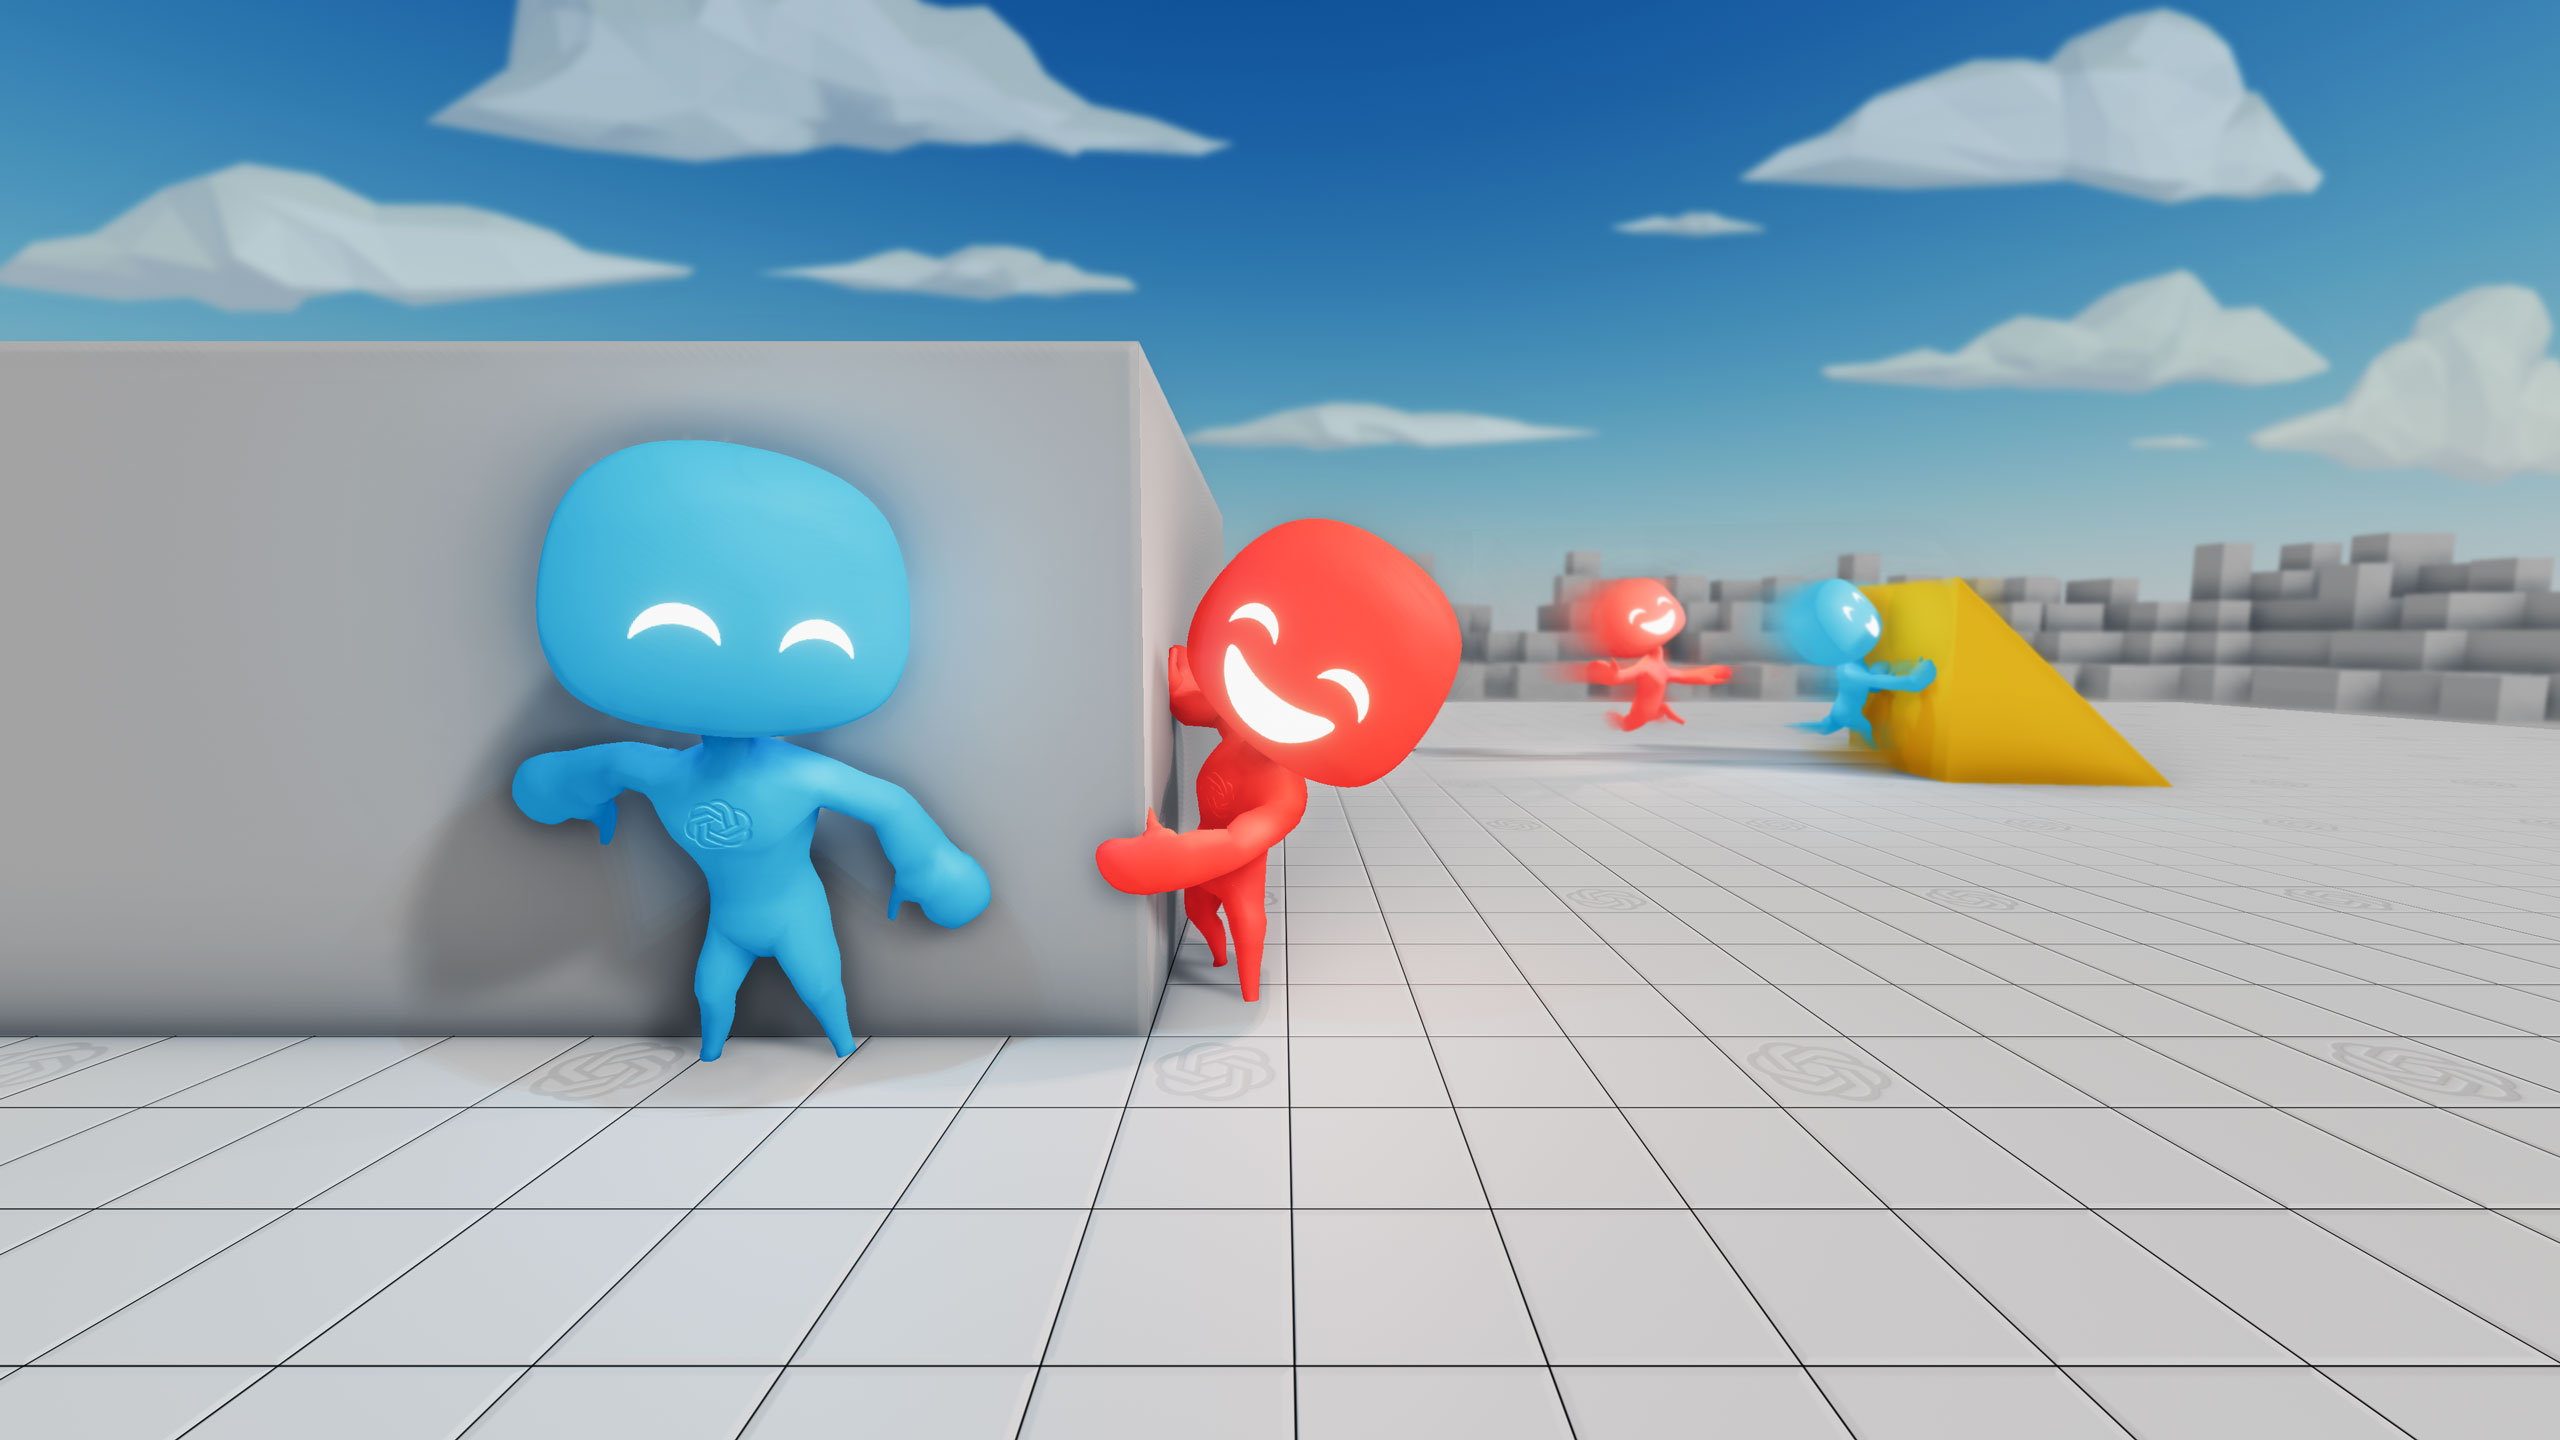
\includegraphics[width=\textwidth]{img/open-ai.jpg}}
		\end{figure}
	\end{exampleblock}
\end{frame}
\begin{frame}[c]{Stochastic Game $\mathcal{S}$ (or Markov games)}
	%/////////
	\begin{alertblock}{Definition}
		\begin{itemize}
			\item $\mathcal{S}$ is a tuple $<N, S, \{A^i\}_{i \in \{ 1, \dots, N\}}, P, \{R^i\}_{i \in \{ 1, \dots, N\}}>$
			\item $N$ is the number of agents ($|N| > 1 $)
			\item $S$ is the global environment state
			\item $A^i$ is the action state of agent $i$. $\mathbb{A} := A^1 \times \dots\times A^N$ is the joint action space
			\item $P: S x \mathbb{A} \rightarrow \mathcal{P}(S)$ is the state transaction. $\mathcal{P}$ is a discrete probabilistic distribution %(associate for each $s \in S$ a probability)
			\item $R^i: S \times \mathbb{A} \times S \rightarrow \mathbb{R}$ is the reward signal
			\item Typical time evolution: $ S_0, \mathbb{A}_0, \mathbb{R}_1, S_1, \dots  $
		\end{itemize}
	\end{alertblock}
	\begin{exampleblock}{Paper Rock Scissor (Repeated)}
		\begin{tasks}(2)
			\task $N = 2$
			\task $A^1 = A^2 = $ \{Paper, Rock, Scissor\}
			\task $S = \{ \mathbb{A}_{t-1} \} $
			\task $R = \begin{blockarray}{cccc}
        & Rock & Paper & Scissor \\
      \begin{block}{c[ccc]}
        Rock    & 0, 0  & -1, 1 & 1, -1 \\
        Paper   & 1, -1 & 0, 0  & -1, 1 \\
        Scissor & -1, 1 & 1, -1 & 0, 0 \\
      \end{block}
    \end{blockarray}$
		\end{tasks}
	\end{exampleblock}
\end{frame}
\begin{frame}[allowframebreaks]{Learning in Multi Agent Environment / Stochastic Games}
\begin{exampleblock}{Task type}
	\begin{itemize}
		\item \textbf{Cooperative}
		\begin{itemize}
			\item Agents share the same reward function ($R^1 = R^2 = \dots = R^N$) or the same collective goal
			\item Examples: multi-agent pathfinding, multi-agent resource allocation, multi-agent task allocation, \dots
		\end{itemize}
		\item \textbf{Competitive}
		\begin{itemize}
			\item Agents compete with each other to maximise a long-term return
			\item Examples: Boards games, battle games, \dots
		\end{itemize}
	\end{itemize}
\end{exampleblock}
%%%%
\begin{exampleblock}{Policy Type}
\begin{itemize}
	\item \textbf{Homogeneous}
	\begin{itemize}
		\item Each agent has the same action space ($ A^1 = A^2 = .. A ^N$) and use the \textbf{same} policy ($ \pi^0 = \pi^N$)
		\item Used in \emph{cooperative} settings and with many agent interactions (e.g., swarm robotics)
		\begin{itemize}
			\item Complexity emerges from interactions
		\end{itemize}
		\item Examples (swarm robotics): obstacle avoidance, flocking, team formation, \dots
	\end{itemize}
	\item \textbf{Heterogeneous}
	\begin{itemize}
		\item Each agent has a different action space ($ A^1 \neq A^2 \neq .. A ^N$) and use a \textbf{different} policy ($ \pi^0 \neq \pi^N$)
	\end{itemize}
\end{itemize}
\end{exampleblock}
%%%%
\begin{exampleblock}{Communication constraints}
\begin{itemize}
	\item \textbf{Independent}
	\begin{itemize}
		\item The policy of each agent is independent of the policy of the other agents
		\item Cooperation could emerge through environment dynamics (but is hard)
	\end{itemize}
	\item \textbf{Joint Action}
	\begin{itemize}
		\item The policy of each agent depends on the action of the other agents ($ \pi(s_t, a^{-i}_t)^i $, where $-i$ means the other agents' indices)
		\item Cooperation is explicitly encoded in the policy
		\item Action space exponentially increases with the agent population
	\end{itemize}
\end{itemize}
\end{exampleblock}
%%%%
\begin{exampleblock}{Execution constraints}
\begin{itemize}
	\item \textbf{Centralised}
	\begin{itemize}
		\item A central controller is responsible for the execution of the policy
		\item It has a global view of the environment and can coordinate the agents
	\end{itemize}
	\item \textbf{Decentralised}
	\begin{itemize}
		\item Each agent executes its own policy
		\item They don't have a global view of the environment, but (potentially) they can communicate
	\end{itemize}
\end{itemize}
\end{exampleblock}
%%%%
\begin{exampleblock}{Learning constraints}
\begin{itemize}
	\item \textbf{Centralised}
	\begin{itemize}
		\item A central agent is responsible for the learning process
		\item It could produce centralised or decentralised policies
	\end{itemize}
	\item \textbf{Decentralised}
	\begin{itemize}
		\item Each agent has its own learning process
		\item It mainly produces decentralised policies
	\end{itemize}
\end{itemize}
\end{exampleblock}

\begin{alertblock}{Big Question: Can we use Single Agent RL in MAS?}
\begin{itemize}
	\item It depends on the \emph{task type}, \emph{policy type}, \emph{communication} constraints, \emph{execution} constraints, and \emph{learning} constraints
	\item Single agent RL could be easily adapted in some cases:
	\begin{itemize}
		\item Task type: cooperative
		\item Policy type: homogeneous
		\item Communication constraints: independent
		\item Execution constraints: centralised/decentralised
		\item Learning constraints: centralised/decentralised
	\end{itemize}
	\item In other cases, they could fail easier
\end{itemize}
\end{alertblock}
\end{frame}
\section{Conclusion}
\begin{frame}[shrink=5]{Conclusion}
	\begin{block}{What we have learned}
		\begin{itemize}
			\item Deep Reinforcement Learning is a powerful tool for solving complex tasks
			\item Multi-Agent Reinforcement Learning extends the capabilities of RL to multi-agent systems 
		\end{itemize}
	\end{block}
	\begin{exampleblock}{Just a scratch on the surface}
		\begin{itemize}
			\item Both topics are vast and complex and they are still under active research
			\item To generalist agents \faArrowRight \, foundational model and GAI?
			\item To large scale \faArrowRight \, many-agent RL?
		\end{itemize}
	\end{exampleblock}
	\begin{block}{Resources}
		\begin{itemize}
			\item \citetitle*{10.5555/3312046}: intro to Reinforcement Learning (reference book)
			\item \citetitle*{zai2020deep}: practice oriented book on Deep Reinforcement Learning
			\item \citetitle*{graesser2019foundations}: intro to Deep Reinforcement Learning
			\item \emph{Multi-Agent Reinforcement Learning}: \url{https://www.marl-book.com/}
		\end{itemize}
	\end{block}
\end{frame}
%/////////
	
%===============================================================================
\section*{}
%===============================================================================

%/////////
\frame{\titlepage}
%/////////

%===============================================================================
\section*{\refname}
%===============================================================================

%%%%
\setbeamertemplate{page number in head/foot}{}
%/////////
\begin{frame}[c,noframenumbering, allowframebreaks]{\refname}
%\begin{frame}[t,allowframebreaks,noframenumbering]{\refname}
	\tiny
	\nocite{*}
	\printbibliography
\end{frame}
%/////////

%%%%%%%%%%%%%%%%%%%%%%%%%%%%%%%%%%%%%%%%%%%%%%%%%%%%%%%%%%%%%%%%%%%%%%%%%%%%%%%%
\end{document}
%%%%%%%%%%%%%%%%%%%%%%%%%%%%%%%%%%%%%%%%%%%%%%%%%%%%%%%%%%%%%%%%%%%%%%%%%%%%%%%%
